\section{The R\lowercase{e}D Experiment}
\label{sec:Red}

The \ReD\ project aims to characterize the light and charge response of a \LArTPC\ to 
neutron-induced nuclear recoils, especially at low energy, and to explore for the possible 
directional dependence suggested by the \SCENE\  experiment~\cite{Alexander:2013ke,Cao:2015ks}. 
\ReD\ consists in the irradiation of a miniaturized \LArTPC\ with a neutron beam at the 
INFN, Laboratori Nazionali del Sud (LNS), Catania. 
Neutrons are produced via the reaction p($^{7}$Li,$^7$Be)n from a primary $^{7}$Li beam 
delivered by the TANDEM accelerator of LNS. A $\Delta$E/E telescope, made by two 
Si detectors, identifies the charged particles ($^{7}$Be) which accompany the 
neutrons emitted towards the \TPC. Neutrons scattered from the \TPC\ are detected by 
using an array of nine \RedLNSNeutronSpectrometerDetectorsPMTsDiameter\ liquid scintillator 
(LSci) detectors,  using \RedLNSNeutronSpectrometerDetectorsScintillatorType\ liquid 
scintillator coupled to \RedLNSNeutronSpectrometerDetectorsPMTsType\ \PMTs.  The \ce{Si} 
telescope and the \TPC\ are not at the same height: this is required in order to tag 
neutron scatterings (n,n') from a non-horizontal interaction plane. All LSci are placed 
such to tag recoils having the same energy, i.e. the same scattering angle with respect 
to the incident neutron, but different angle with respect to the drift field of 
the \LArTPC, thus allowing to search for a possible directional response. A schematic 
layout of the experiment is displayed in Fig.~\ref{fig:ReD-sketch}. \\
\begin{figure*}
\centering
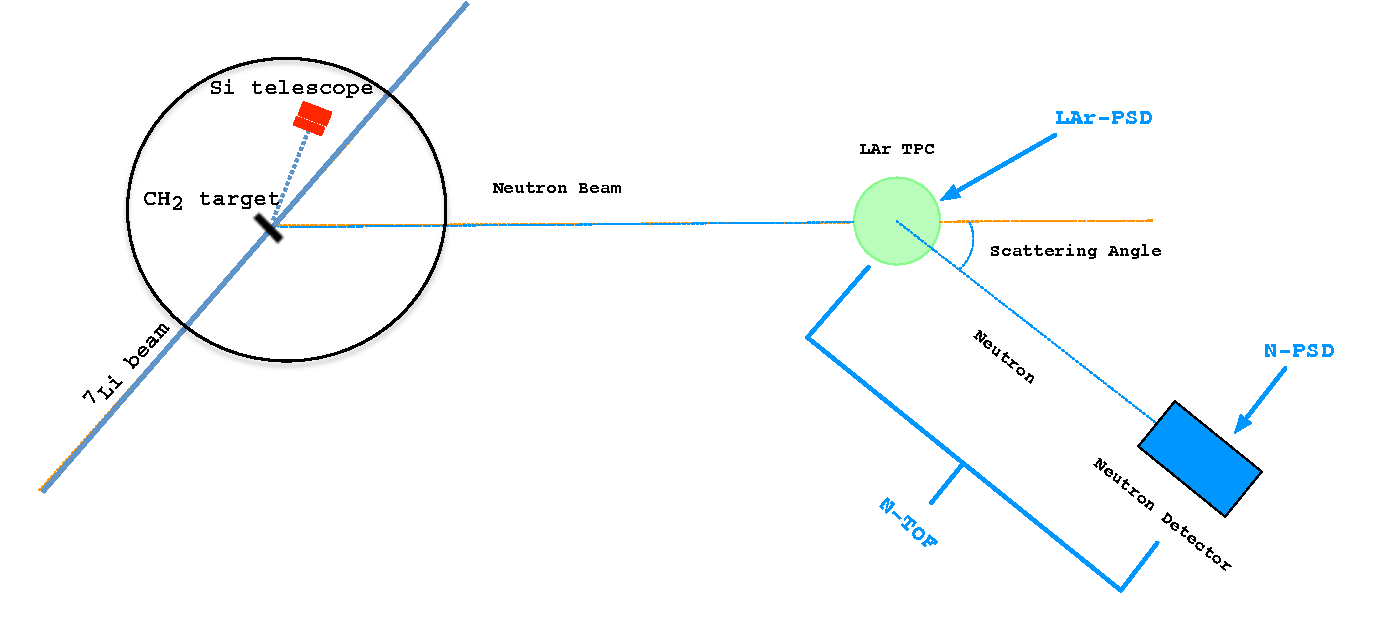
\includegraphics[width=0.85\textwidth]{./Figures/ReD-Sketch.pdf} 
\caption{Schematic drawing of the \ReD\ experimental set-up.}
\label{fig:ReD-sketch}
\end{figure*}

The core detector of \ReD\ is a custom-made \TPC\ designed by UCLA, which is a miniaturized 
version of the \LArTPC\ for \DSks.  The \TPC\ is a cube with size of about 
\GAPTPCActiveDiameter.  An acrylic vessel defines the active volume, with the top and 
bottom acrylic windows \ITO\ coated to allow for the application of the electric field, and the 
side ESR-acrylic sandwich reflection panels to maximize the reflectivity of the chamber. 
All of the internal surfaces are coated with TPB to wavelength shift the argon scintillation 
light. The drift field is kept uniform along the drift coordinate by means of the field shaping 
rings, deposited by thin-coating the walls of the acrylic vessel with \ITO. The drift 
length, extraction length and electroluminescence length of the \ReD\ \TPC\ are 5~cm, 3~mm 
and 7~mm, respectively. The \ReD\ \TPC\ uses all the innovative features of the \DSks\ 
design, in particular the optoelectronic readout based on \SiPM\ developed by FBK and the 
cryogenic electronics. Two 5x5~cm$^2$ tiles are available from FBK, each made by 24 
rectangular \SiPMs.  The tile on the top of the \LArTPC\ has a 24-channel readout, in order 
to improve the $(x,y)$ sensitivity, while the bottom tile has a standard 4-channel readout.  
A dedicated 24-channel Front End Board (FEB) has been designed and produced by INFN-Na in 
collaboration with INFN-Bo and LNGS. After the commissioning of the cryogenic system 
in Naples and an initial characterization with lasers and low-energy $\gamma$ sources, 
the set-up was shipped to Catania in June 2018. \\

Thanks to the support provided by INFN CSN2, the full \ReD\ system was integrated, and deployed 
to the ``80 deg'' beamline of LNS for a first test beam, which took place in June-July 2018. 
The beamline had been previously refurbished on the basis of the experimental design, 
optimized with dedicated Monte Carlo simulations, and the mechanical clearance requirements. 
The configuration was conceived to allow the tagging of nuclear recoils between 20 and 100~keV 
traveling in the parallel and orthogonal directions with respect to the \TPC\ drift field, 
by varying the primary beam energy only. Furthermore, having a dedicated liquid 
scintillator at small scattering angles opens the possibility to study the response of the 
\TPC\ to very low-energy nuclear recoils, O(1~keV).  A new scattering chamber was 
installed with a new beam pipe. The $\Delta E/E$ telescope was installed inside the 
vacuum scattering chamber and commissioned; it consists of two Si detector (20 $\mu$m and 
200 $\mu$m thickness, respectively) by ORTEC. The nine LSci detectors had been previously 
tested and characterized at INFN-Roma1.
Initially, the cryostat and the liquid scintillators had to be mechanically aligned with respect 
to the target point with a precision of the order of a few mm. The alignment was performed by 
following a detailed procedure worked out in advance. The \ReD\ set-up in Catania is 
displayed in Fig.~\ref{fig:BeamlinePhoto}. 

\begin{figure}[t!]
\centering
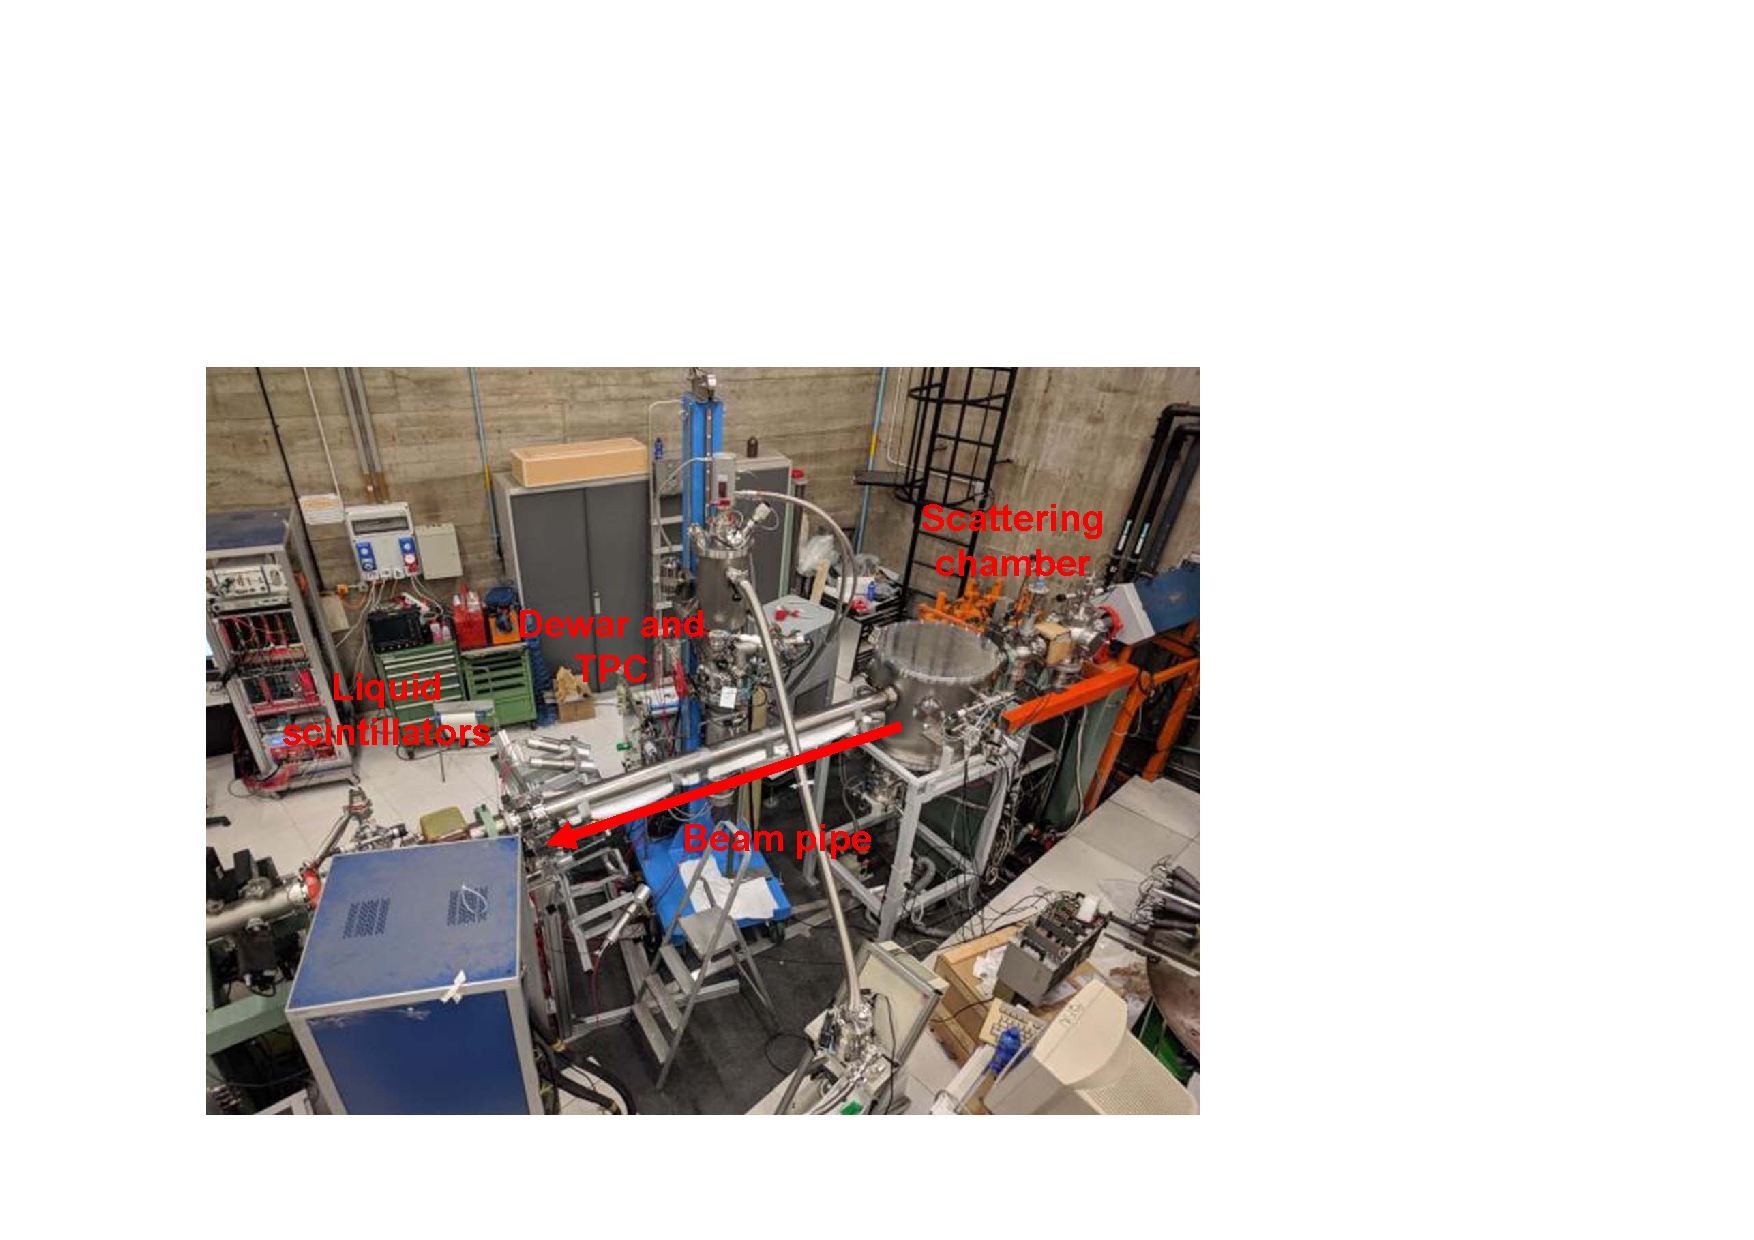
\includegraphics[width=0.7\columnwidth]{./Figures/BeamLineDisplay.pdf}
\caption[Picture of the \LNS\ beamline in use for \ReD]{Photo of the ``80 deg'' 
beamline at \LNS, after the deployment and alignment of \ReD.  The targets and the Si 
telescope are hosted inside the vacuum scattering chamber.}
\label{fig:BeamlinePhoto}
\end{figure}

The test beams aimed at the integration of the three detector systems with the TANDEM beam, which 
also included operating procedures, photosensors, \DAQ, slow control, data handling and 
reconstruction algorithms. The new LabVIEW-based slow control developed by INFN-Genova was 
integrated and commissioned. Neutrons were produced by sending a $^{7}$Li 28~MeV beam 
onto a set of CH$_2$ targets having thickness between 150 and 250~$\mu$g/cm$^2$. 
The intensity of the beam impinging on the target after the collimator ranged between 0.5 
and 7~nA. The \DAQ\ software handled 41 readout channels from three FADC boards (CAEN~V1730), 
at 500 MHz sampling rate. The Si telescope was placed at 5~deg with respect to the beam. 
The scattering kinematics allows for two solutions 
with $^{7}$Be in this direction, one having an associated 7.5~MeV neutron at 22.5~deg, 
the other with a 2~MeV neutron at 45~deg. The \LArTPC\ is at 22.5~deg from the target, 
i.e. it is hit by 7.5~MeV neutrons, produced in association with the $^{7}$Be detected by the 
Si telescope. The beam energy and the scattering angles cause the experiment to select 
nuclear recoils in the \TPC\ of approximately 70~keV.
About 24 hours of data have been taken in the best operating conditions, split in single and 
double phase modes. Events were observed with the proper signature, i.e. a $^{7}$Be nucleus 
detected by the telescope, a nuclear recoil in the \LArTPC\ and a neutron scattering in the 
liquid scintillators. Neutron-induced recoils events in the \TPC\ and in the LSci 
detectors are clearly separated from $\gamma$ signals, either physical or accidental,
by means of pulse shape discrimination.\\ 

After another LNS test beam in September 2018, the \ReD\ \TPC\ was transported back to 
Naples, to complete the characterization and re-commissioning. Tests were
performed to characterize the basic TPC performance in terms of light yield, 
uniformity, electric field configuration and \STwo/\SOne\ ratio in double phase. The system was 
calibrated with laser, $\gamma$-sources, an internal $^{83m}$Kr source 
(which generates a uniform distribution of mono-energetic events), and neutrons. 
Neutrons were produced from a DD generator from the Temple University, in order to assess the 
ER/NR discrimination capability of the \TPC. 
The electric field configuration was optimized such to achieve a performance 
which is suitable for the measurement at the beam; specifically, the drift field is set 
at 200~V/cm, which gives a maximum drift time of about 60~$\mu$s, and the extraction 
field at 5.8~kV/cm. Fig.~\ref{fig:TPCperformance} displays the distributions of \SOne\ and 
of $\langle S2/S1 \rangle$ obtained with an $^{241}$Am source. The light yield at null 
field is about 10~phe/keV. The energy resolution $\sigma/\mu$ achieved at 59.5~keV by 
using a dedicated algorithm for digital filtering of the waveforms is 5.4\% (plain 
charge integration gives $\sigma/\mu \sim 6\%$). The spatial uniformity of the \TPC\ response 
was also tested with a $^{83m}$Kr source dissolved in \LAr: it is within 15\% in $xy$ and 
at the few percent level in $z$. The \SOne\ and drift time distributions from $^{83m}$Kr 
are displayed in Fig.~\ref{fig:ReDUniformity}: the uniformity of the drift time profile 
is an indication of the very good uniformity of the drift field along the \TPC. 
%
\begin{figure}[tbp!]
\centering
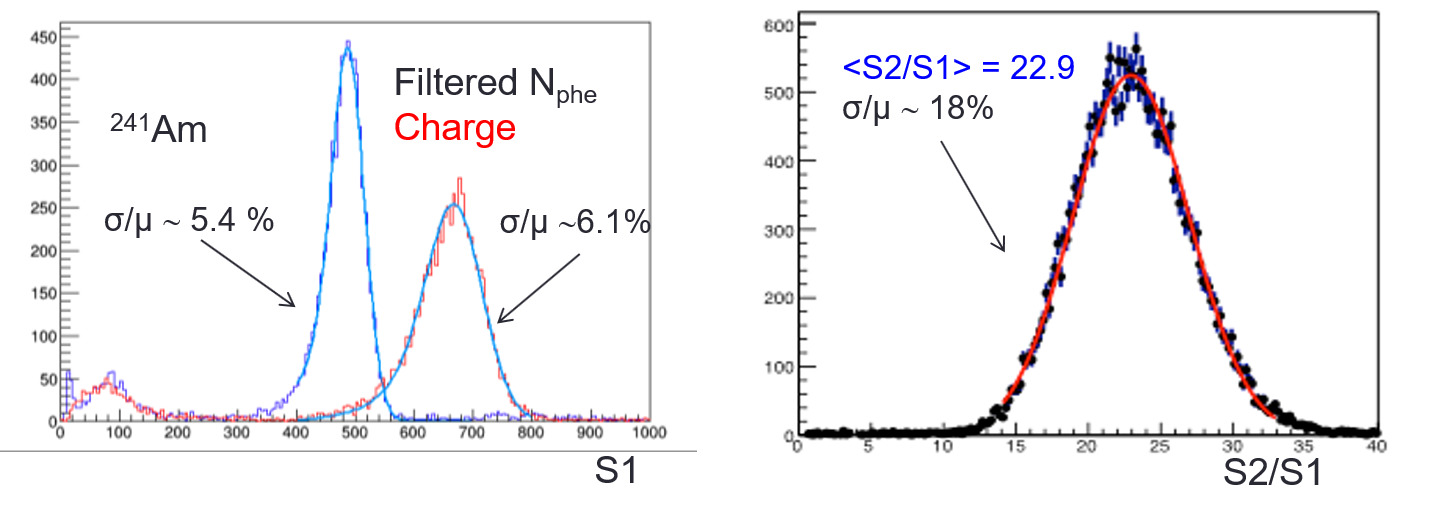
\includegraphics[width=0.95\columnwidth]{./Figures/TPCperformance.png}
\caption[\ReD\ \TPC\ performance]{S1 and $\langle S2/S1 \rangle$ spectra of the 
\ReD\ \TPC\ irradiated with a $^{241}$Am $\gamma$ source, to show the performance in terms of light 
and charge. Drift field is set at 200~V/cm and extraction field at 5.8~kV/cm.}
\label{fig:TPCperformance}
\end{figure}
%
\begin{figure}[tbp!]
\centering
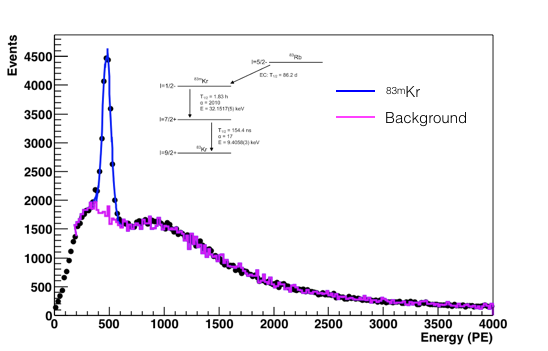
\includegraphics[width=0.46\columnwidth]{./Figures/kr_973.png}
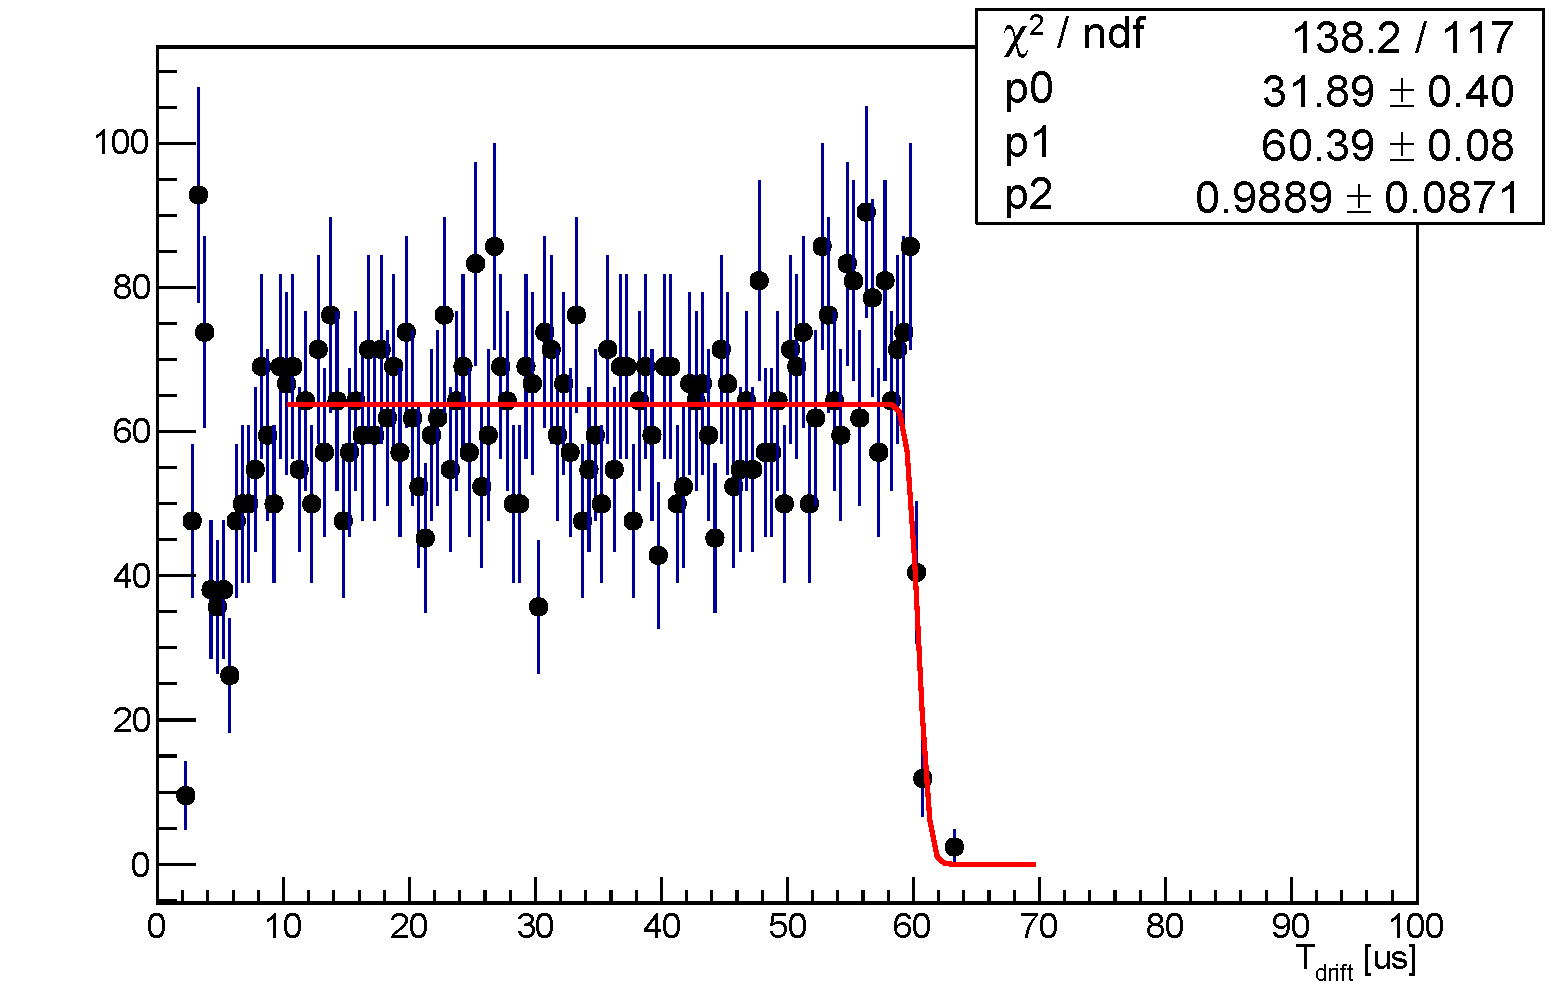
\includegraphics[width=0.44\columnwidth]{./Figures/Kr_standardField_TdriftFit.png}
\caption[\ReD\ \TPC\ \SOne\ and drift time with $^{83m}$Kr]{S1 (left) and drift time (right) distributions 
obtained by dispersing a $^{83m}$Kr source in the \ReD\ \TPC.}
\label{fig:ReDUniformity}
\end{figure}
%
The electron lifetime is $> 500 \mu s$, i.e. much longer than the maximum drift time in the \TPC, 
with no hints of degradation in time. The anti-correlation between the scintillation and charge yield 
for drift fields between 0 and 1000~V/cm is displayed in Fig.~\ref{fig:reddoke}; a charge 
yield of about 16~phe/e- is achieved in the current configuration. \\
\begin{figure}[tbp!]
\centering
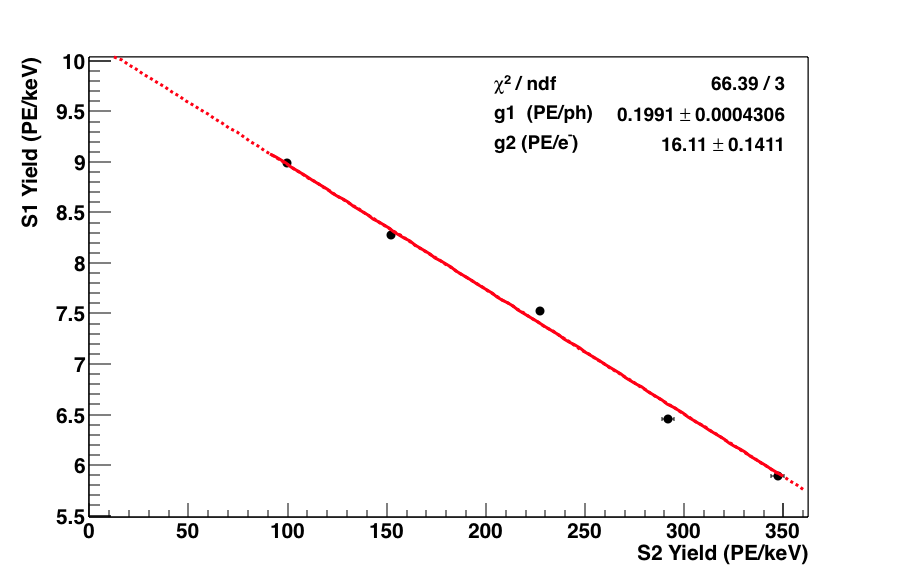
\includegraphics[width=0.6\columnwidth]{./Figures/asy_s1_s2_finale_s2fitmod_no0.png}
\caption[\SOne-\STwo\ anti-correlation in \ReD]{Anti-correlation between light and charge signal in the 
\ReD\ \TPC\ for drift fields ranging between 0 and 1000~V/cm.}
\label{fig:reddoke}
\end{figure}

A campaign was also carried out at LNS to characterize the performance of the liquid 
scintillators and the absolute neutron detection efficiency by using a fission $^{252}$Cf 
source.  A \SI{50}{\percent} trigger efficiency at 20~keV$_{ee}$ and a time resolution of 0.5~ns 
(rms) were demonstrated, that is largely sufficient for the measurement of the 
time-of-flight. The absolute neutron efficiency was found to be between 20 and 30\% in the 
energy range 1-10~MeV of interest for \ReD, in agreement with the Monte Carlo 
expectations.

Two test beams with $^{7}$Li were performed in 2019 at LNS in Catania, aiming to improve the beam configuration 
and to characterize the neutron beam. In these tests, only the Si telescope and the liquid 
scintillators were operated. A remotely-controlled motor was installed within the scattering 
chamber and commissioned: this allows for the precise movement of the telescope, 
thus providing an additional tool for the fine-tuning of the alignment and for the compensation 
of possible small misplacements from the mechanical procedure. Beam current of 10 to 20~nA were 
routinely achieved on CH$_2$ targets of thickness between 300 and 400~$\mu$g/cm$^2$. Thanks 
to the better alignment and the more intense beam, the expected rate of three-fold 
coincidence is hence expected to increase by a factor of $> 10$ with respect to the test 
beams of 2018.

The \ReD\ project has received scientific approval by the Scientific Committee of LNS (PAC) 
for a five-week beam allocation that is granted for 2019-2020.  The \ReD\ \LArTPC\ is 
expected to be transported back to Catania before the end of 2019, for a new test beam with 
the full set-up. Upon successful completion of such a test, several one-week-long beam 
slots will be scheduled to perform the physics measurement.

